\documentclass{utue} %utue.cls required for Uni Tuebingen corporate design

\usepackage[style=alphabetic, maxbibnames=99]{biblatex}
\addbibresource{bibliography.bib}
\usepackage{amsmath}
\usepackage{placeins}
\usepackage[hidelinks]{hyperref}

% Values for title generation
\title{Controlling Phasor Noise Artifacts}
\author{Jonathan Lang}
\date{\today}

% Subtitle is optional. It represents what kind of work you did.
\subtitle{Research Project}

\hypersetup{
  colorlinks=false,
  pdftitle={Controlling Phasor Noise Artifacts},
  bookmarks=true,
}

\DeclareMathOperator{\atan}{atan}

\begin{document}

% You can place a teaser as follows. (Otherwise, just uncomment the following part)
%\teaser{
%    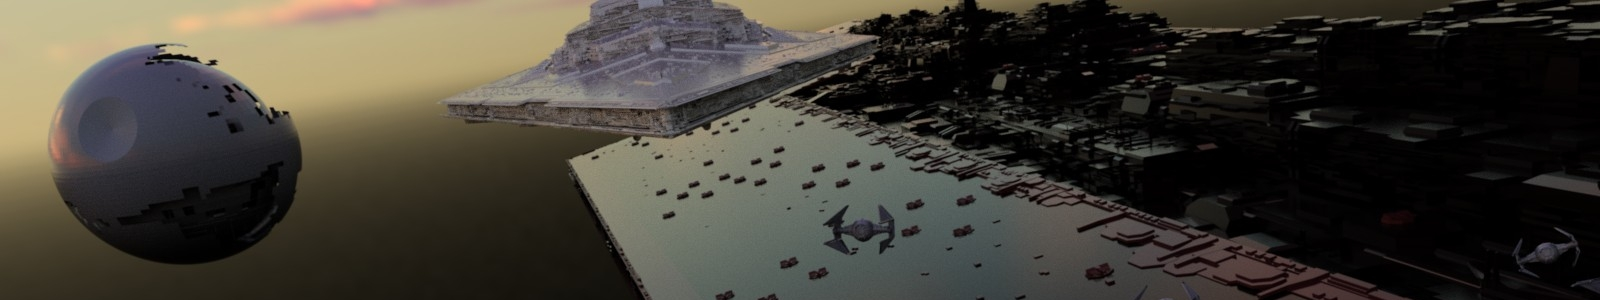
\includegraphics[width=\textwidth]{images/teaser.jpg}
%    \caption{\label{fig:teaser}You can place a teaser here.}
%}     

% Creates title of document and additional title page.
\maketitle 
 
\section*{Abstract}  
Procedural Phasor noise is a powerful tool to synthesize normalized noise patterns. However, it also generates artifacts in the form of singularities and rips. We present a method generate a bilobe Phasor Noise instance only containing defined artifacts by synthesizing the phase directly instead of constructing it using the corresponding Gabor noise Instance. We also start development on a method for more complex cases and show how our method can be expanded to surface noise.
  
\section{Introduction}   
To keep up with the shorter development cycles of the current times, more work has to be done in less time. The tools with which this is achieved are optimization of workflows as well as automation. While even the automation of repetitive tasks can be challenging, automating creative tasks like content creation is even more so. This is where noise algorithms provide assistance. They provide a way to generate non-repeating patterns over potentially infinite space at low memory and computational cost. Using these patterns to influence different aspects of the content, anything from additional detail on surfaces up to the layout of whole worlds can be generated automatically. The generated patterns are as varied as the algorithms itself. The different algorithms also provide different levels of influence over the produced pattern. Additional parameters to tune the generated pattern are of course desirable, as a richer set of patterns will be applicable to more situations, therefore offering further automation opportunities.


\section{Related Work}
Particularly interesting are anisotropic noise algorithms. As stated in \cite{survey}, these noise algorithms produce patterns, whose appearance is not invariant to rotation. Besides providing definitions of most noise related terms, \citeauthor{survey} also provide an overview of current Noise algorithms. The noise algorithm proposed by \citeauthor{anisotropicNoise} in \cite{anisotropicNoise} is actually not developed to produce interesting patterns with a discernible direction, but to enable the production of filtered noise to prevent aliasing when the noise texture is viewed at an angle. Today, the term \textit{anisotropic noise} is more commonly used to refer to noise algorithms, which set out to produce oriented patterns instead of ones with integrated filtering. One of these algorithms is the one proposed by \citeauthor{randomPhaseNoise} in \cite{randomPhaseNoise}. \citeauthor{randomPhaseNoise} produce noise by placing cosine functions with random phase, direction and frequency at grid points. By adjusting the way these random values are generated, the power spectrum of the noise can be controlled precisely. The ability to precisely control the power spectrum is a property shared with Gabor Noise as introduced by \citeauthor{gaborNoise} in \cite{gaborNoise}. Gabor Noise is a sparse convolution noise using a Poission point process to generate Dirac impulses that are convoluted with the Gabor kernel to produce the final noise. Since this process inherits the power spectrum of the Gabor kernel, which can be adjusted quite precisely, this affords good control over the power spectrum of the noise, especially when differing instances of the kernel are used. This is a property leveraged in \cite{gaborNoiseByExample} to generate noise that mimics given textures. Despite of how powerful Gabor noise is, it is still not perfect. One problem it exhibits are the areas of low contrast, that have never been explicitly specified. This is a conclusion \citeauthor{spectrumOfVariance} also come to. In \cite{spectrumOfVariance} they develop a tool to quantify this local loss of contrast, which they call the spectrum of variance. Based on this, they develop a technique to remove low contrast areas from any noise instance. This generality, however, is a drawback as much as an advantage, since it can not use any information about the noise generation to achieve lower computation times. This is exactly what \citeauthor{phasorNoise} do in \cite{phasorNoise}. We will later have a more in depth look at their work.\\
Another big advantage of Gabor noise is its ability to be generated on the surface directly. This does not involve any texture coordinates, so the resulting noise instance does not show any seams. This ability is sought for, as works like \cite{appearanceTextureSynthesis}, \cite{textureSynthesis} and \cite{stripes} show. The former present algorithms that can synthesise textures directly on surfaces, while the latter addresses a more basic problem. This problem is to find a function on a surface that varies along a given direction field with a given rate. This is another piece of work we will look at in the following section.

\section{Background}
To avoid confusion, we will denote a scalar using a simple letter e.g. $a$. A vector will be denoted with an arrow above e.g. $\vec{u}$. A scalar or elementwise multiplication will be represented by $\cdot$ or the absence of an operator e.g. $a\cdot b=ab$ is the multiplication between $a$ and $b$. The operands of a scalar product will be surrounded by $\langle$ and $\rangle$ e.g. $\langle\vec{u},\vec{v}\rangle$ denotes the scalar product between the vectors $\vec{u}$ and $\vec{v}$.

\subsection{Gabor Noise}
Since Phasor Noise inherits most of the abilities of Gabor Noise, we will have a look at Gabor Noise before discussing it. As already mentioned, Gabor Noise is produced by convolving Dirac impulses placed by a Poisson point process with the Gabor kernel as shown in Figure \ref{fig:gaborNoise}. The Gabor kernel $g$ is defined as
$$
g(\vec{x}) = e^{\frac{||\vec{x}||}{\sigma^2}}\cdot \cos{(f\langle\vec{u},\vec{x}\rangle)},
$$
where $f$ and $\vec{u}$ are frequency and direction of the kernel and $\sigma$ represents its width like it does for a Gaussian function. Since the other operand of the convolution is a sum of offset Dirac impulses, the convolution deteriorates to a sum of offset versions of the kernel. An instance of Gabor Noise $G$ can therefore be represented as
$$
G(\vec{x}) = \sum_ig(\vec{x}-\vec{p}_i),
$$
where $\vec{p}_i$ are the positions of the Dirac Impulses. \citeauthor{gaborNoise} also prescribe a random weight to each instance of the kernel. However, since this is not relevant for the following discussion, we omit it here for convenience. Figure \ref{fig:gaborNoise} shows an instance of Gabor Noise. The depicted instance is a bilobe instance. This name stems from the appearance of its power spectrum, which is two Gaussian lobes positioned at the frequency and direction of the used kernel. Using different kernels at different positions leads to a more varied appearance. Since the power spectra add up (and are rescaled) this permits to specify a custom power spectrum. Besides this amount of control, Gabor noise can of course be extended from two to three dimensions. However, \citeauthor{gaborNoise} also present a way to generate Gabor Noise directly on the surface of objects, which allows for seamless texturing.

\begin{figure}[ht]
  \centering
  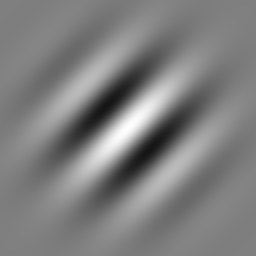
\includegraphics[width=0.49\linewidth]{images/gaborKernel}
  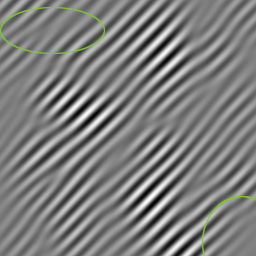
\includegraphics[width=0.49\linewidth]{images/gaborNoise}
  \caption{An instance of the Gabor Kernel (left) and an instance of Gabor Noise (right). Note the low contrast areas, like the ones that are marked.}\label{fig:gaborNoise}

\end{figure}

\subsection{Spectrum of Variance}
Gabor Noise exhibits areas of low contrast, as Figure \ref{fig:gaborNoise} shows. In \cite{spectrumOfVariance} \citeauthor{spectrumOfVariance} develop a tool to quantify these areas. They call this tool the spectrum of variance. As the name suggests for a given signal $s(\vec{x})$ the spectrum of variance $\mathcal{S}(s)$ is defined as
$$
\mathcal{S}(s) = \mathcal{F}((s-\overline{s})^2),
$$
where $\mathcal{F}$ denotes the Fourier transform and $\overline{s}$ represents the mean of the signal. Any nonzero values nearer than a distance $l$ to the origin correspond to low contrast areas bigger than $l$ in the original signal. This can be seen, when comparing Figure \ref{fig:gaborNoise} and \ref{fig:phasorNoise} alongside with Figure \ref{fig:spectrumOfVariance}. They also propose a process to remove these low contrast areas, namely by normalizing with the windowed standard deviation. However, this normalization requires to compute the windowed standard deviation, which requires the evaluation of the noise in the used window. This leads to a big increase in computational cost, which is a significant drawback of this technique.

\begin{figure}[ht]
  \centering
  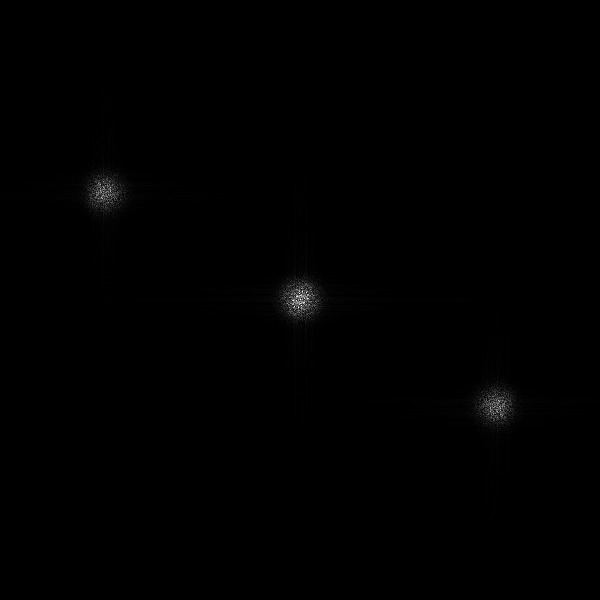
\includegraphics[width=0.49\linewidth]{images/gaborNoiseSpectrumOfVariance}
  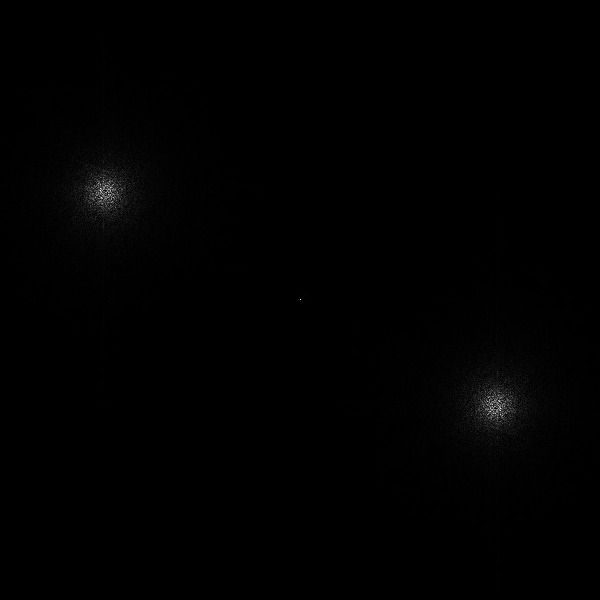
\includegraphics[width=0.49\linewidth]{images/phasorNoiseSpectrumOfVariance}
  \caption{The spectrum of Variance of Gabor noise (left) and Phasor noise (right) as displayed in \cite{phasorNoise}. Note the absence of a central lobe for Phasor Noise, which indicates no local loss of contrast.}\label{fig:spectrumOfVariance}
\end{figure}

\subsection{Phasor Noise}\label{sec:phasorNoise}
The drawback of using the windowed variance for normalization stems from the fact, that they can not use the noise algorithm's internal information. The logical conclusion is, that the only way to get a normalized noise texture without a big computational overhead is to design a variation of the algorithm, that produces normalized images. This is exactly what \citeauthor{phasorNoise} do in \cite{phasorNoise} for Gabor Noise. They realize, that for a signal of the form $s(x) = f(x)\cdot g(x)$, where $g$ is an oscillating function and $f$ is the envelope of $s$, discarding $f$ leads to a perfectly normalized signal. They then proceed to reformulate the bilobe case of Gabor Noise to have the form
$$
G(\vec{x}) = I(\vec{x})\sin{(f\langle\vec{x},\vec{u}\rangle + \varphi(\vec{x}))},
$$
where $f$ and $\vec{u}$ are again the frequency and direction of the main oscillation. $I$ is the envelope of the function and $\varphi(\vec{x})$ is the local phase offset of the oscillating part. $I$ and $\varphi$ are defined in such a way, that this formulation is exactly equivalent to the corresponding Gabor Noise instance. The main tool they use to do this is phasor addition, hence the name Phasor Noise. Now, like in our example, we can discard the envelope $I$ to obtain a normalized version of Gabor Noise. \citeauthor{phasorNoise} call this a phasor sine wave. The actual Phasor Noise is the argument of the sine. Therefore, Phasor Noise itself can not be used directly, but can only be used as input for a periodic function. Because it is defined using its corresponding Gabor Noise instance, it inherits the desirable properties of Gabor Noise, namely being band limited and a surface noise formulation. However, as depicted in Figure \ref{fig:phasorNoise}, Phasor Noise exhibits several artifacts previously masked by the low contrast areas. There are two types of artifacts: singularities, where one stripe splits into two and what we will call rips, where the stripes are suddenly offset by some amount. With our method, control can be gained over these artifacts to allow for finer adjustments to the appearance of the noise.

\begin{figure}[ht]
  \centering
  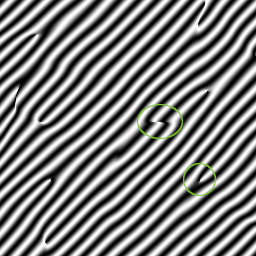
\includegraphics[width = 0.49\linewidth]{images/phasorSineWave}
  \caption{A Phasor sine wave. Note the artifacts previously masked by the low contrast areas.}\label{fig:phasorNoise}
\end{figure}

\subsection{Stripes Patterns on Surfaces}
In Section \ref{sec:stripes}, we will see, that we need a function $F$, defined on a mesh, that increases with a direction $X$ and speed $\nu$ determined by a vector field. We need this function to generate a stripe pattern by plugging it into a periodic function. One way to compute this function is as the integral over the direction field. As stated in \cite{stripes}, this is not always possible, even for a simple plane, as vector fields with non-zero curl are non-integrable. \cite{stripes} also provides a solution. They achieve this by trying to find a complex function $\psi$, whose argument $\alpha$ is equal to $F$. Constraining $d\alpha(Y) = \nu\langle X,Y\rangle$ leads them to differential equation for $\psi$. In most cases this equation does not have a solution, so they relax this constraint to a minimization and obtain a complex version of the Dirichlet energy. They then proceed to minimize this energy akin to the normal Dirichlet energy. While necessary to receive a solution, this minimization unfortunately allows new singularities to emerge, which is obviously necessary, when considering an object whose width varies along the stripe direction. As the width the stripes have to cover increases, either the number of stripes needs to increase, or the stripe frequency needs to drop. For our application, one could replace their work with another way to generate a function that increases according to a vector field, but here we will use their work.

\section{The constant Case}
We will first look at a simple case. This case corresponds to the bilobe case of Phasor Noise. This means a constant oscillation direction and frequency. However, before we start out, we will define a third type of artifact besides singularities and rips: wobble. Comparing the areas of a Phasor sine wave with a regular sine wave, we find that the lines are not perfectly straight. We will refer to this fact as wobble from now on. From Section \ref{sec:phasorNoise} we recall that in this case Phasor Noise consists of two parts: A function increasing in a given direction and a phase offset. Figure \ref{fig:phasorNoisePhase} shows a Phasor Noise instance as well as its phase offset. Comparing the phase from Figure \ref{fig:phasorNoisePhase} with Figure \ref{fig:phasorNoise}, we can easily find a correspondence between artifacts of the Phasor sine wave and features of the phase. The existence of wobble is caused by the fact, that the phase is not constant even in areas, where there are no other artifacts present. \citeauthor{phasorNoise} already identify that rips are caused by sudden value changes in the phase offset, while singularities are located at points around which the phase offset rotates abruptly.\\

\begin{figure}[ht]
  \centering
  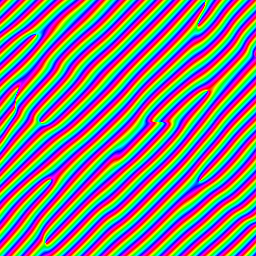
\includegraphics[width=0.49\linewidth]{images/phasorNoise}
  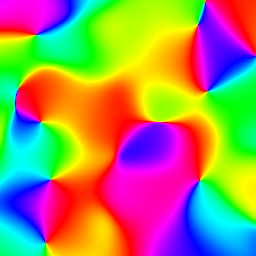
\includegraphics[width=0.49\linewidth]{images/phasorPhase}
  \caption{Phasor Noise (left) and its phase offset (right). Angle is mapped to hue.}\label{fig:phasorNoisePhase}
\end{figure}

This defines our goal: For a set of points $\vec{s}_i$, at which we want singularities to occur and a set of line segments $l_i$, along which we want rips to occur, we want to construct a varying phase offset $\varphi_c$ that suddenly changes when crossing any $l_i$ and abruptly rotates around all $\vec{s}_i$. Since this is a phase offset, the numbers are considered modulo $2\pi$. Since wobble is the artifact most characteristic for Phasor Noise, we will assume that wobble is present in all applications, which will become relevant in Section \ref{sec:singularities}, where we will have a look at how to create singularities. How to actually create wobble will be explained in Section \ref{sec:wobble}. The last artifact type, that is still missing is rips, which will be explored in Section \ref{sec:rips}. After that, we will have a look at adapting these methods to an environment with a non-constant direction field in Section \ref{sec:nonConstant}. Following this is Section \ref{sec:results}, where we will present some applications of the developed methods.

\subsection{Wobble}\label{sec:wobble}
The first kind of artifact we will have a look at is wobble. As already mentioned, wobble is created by a non-constant phase. Since we are creating noise, we want this to be governed by randomness. Taking another look at Figure \ref{fig:phasorNoisePhase}, we can not identify any obvious anisotropy. Therefore, any noise algorithm whose appearance is not obviously anisotropic will be sufficient to create a similar appearance to Phasor Noise. An important thing to note is, that this algorithm does not use the fact, that the output domain is cyclic. There are two reasons for this: The first is, that there is a multitude of noise algorithms with an equally large set of properties, that output to the real domain between $-1$ and $1$.\\
The other, more important one is that it is harder to ensure the absence of singularities when using a cyclic output domain. Take for example a simple algorithm that is based on an integer lattice and at each point of this lattice determines a random number and interpolates between them. Since we are using angles, these random numbers will be between $0$ and $2\pi$. We are on a cyclical domain, so the interpolation will check if the points are nearer when using the normal difference or if they are nearer when computing the difference over the $0$/$2\pi$ boundary and choose the interpolation direction accordingly. We will now construct a possible case, where this algorithm will a create singularity. This case is also shown in Figure \ref{fig:simpleAlgirithmSingularity}. To construct this case, choose a grid cell $C$ and its four corner points $p_1$, $p_2$, $p_3$ and $p_4$ in such a way, that $(p_1,p_2,p_3,p_4,p_1)$ moves along the edges around the cell. Now, let the algorithm pick $0$, $\frac{\pi}{2}$, $\pi$ and $\frac{3\pi}{2}$ for $p_1$, $p_2$, $p_3$ and $p_4$ respectively. Since we interpolate on a cyclical domain, the points on the edge $(p_4,p_1)$ will be assigned values interpolated between $\frac{3\pi}{2}$ and $0$. We therefore created a path with a winding number of $1$ and therefore, according to the argument principle of complex analysis, this path contains a singularity. Note that this problem is not easily fixed without removing the cyclic interpolation.
\begin{figure}[h]
  \centering
  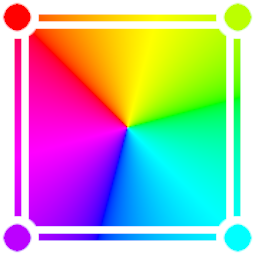
\includegraphics[width=0.49\linewidth]{images/simpleAlgo}
  \caption{A simple noise algorithm creating a singularity on a cyclical domain. The circles represent the points of the lattice while in between them the interpolation is shown. The rest shows possible values for the domain. Angle is again mapped to hue.}\label{fig:simpleAlgirithmSingularity}
\end{figure}

Therefore, we will stick with algorithms outputting to the classic domain of $[-1,1]$. Since we need to scale these value and are using this function to generate angle values, we generate the wobble phase offset $w(\vec{x})$ as
$$
w(\vec{x}) = (a\cdot n(\vec{x}))\ \mathrm{mod}\ 2\pi,
$$
where $a$ determines how much wobble will be added, while $n$ represents the noise function used as a base. Figure \ref{fig:wobble} shows a Phasor sine wave with a phase offset applied. This phase offset is generated using a simple hierarchical algorithm, that uses cosine interpolation between lattice points. Note that while there is an obvious difference in the phase offset used in Figure \ref{fig:wobble} and the phase obtained from real Phasor Noise as shown in Figure \ref{fig:phasorNoisePhase}, there is no noticeable difference in wobble when applied to a Phasor sine wave as shown in Figure \ref{fig:phasorNoise}.
\begin{figure}[h]
  \centering
  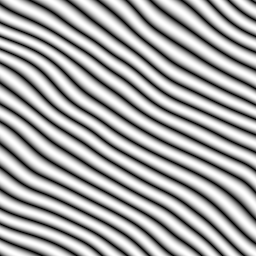
\includegraphics[width=0.49\linewidth]{images/wobble}
  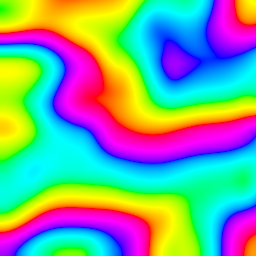
\includegraphics[width=0.49\linewidth]{images/wobblePhase}
  \caption{An artificially created Phasor sine wave (left) without any artifacts except for wobble and its phase offset (right).}\label{fig:wobble}
\end{figure}
When using the function $w(\vec{x})$ to compute the phase offset causing the wobble, we can represent our constructed phase offset as $\varphi_c(\vec{x}) = w(\vec{x})$.

\subsection{Singularities}\label{sec:singularities}
As we already found, singularities are located at points, where the phase offset rotates rapidly. To construct singularities, we therefore need to construct such points in the phase offset. To achieve this, we will (literally) add another component to the generated phase offset. Given the polar coordinates $(r, \theta)$ of a point $\vec{x}$ we can use the function
$$
\atan(\vec{x}) = \begin{cases}
  0 & \text{if } r = 0\\
  \theta &\text{otherwise}
\end{cases}
$$
Figure \ref{fig:singularities} shows this function as well as its impact when used as a phase offset for a sine wave. It also shows $-\atan(\vec{x})$ and its impact when used as phase offset. We can clearly see a difference in the Phasor sine wave. Along the direction from the top left to the bottom right, $\atan(\vec{x})$ leads to an additional line, while $-\atan(\vec{x})$ removes a line. This clearly indicates a need to differentiate between the two. We will call the first one a right singularity, while we will call the second one a left singularity. Recalling from our goal, we want singularities at points $\vec{s}_i$. Since we now need to differentiate between the two types of singularities, we will continue to denote points of right singularities by $\vec{s}_i$, while we will denote points with left singularities by $\vec{t}_i$. Using this, we can expand our constructed phase to
$$
\varphi_c(\vec{x}) = w(\vec{x}) + \sum_i \atan(\vec{x}-\vec{s_i}) - \sum_j \atan(\vec{x}-\vec{t_j})
$$
\begin{figure}[ht]
  \centering
  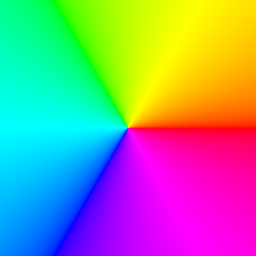
\includegraphics[width=0.235\linewidth]{images/rightSingularityPhase}
  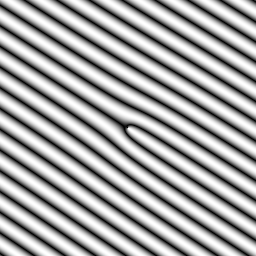
\includegraphics[width=0.235\linewidth]{images/rightSingularity}
  \hfill
  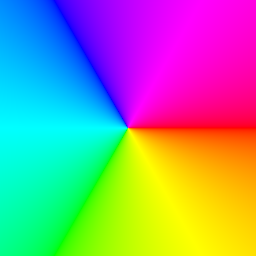
\includegraphics[width=0.235\linewidth]{images/leftSingularityPhase}
  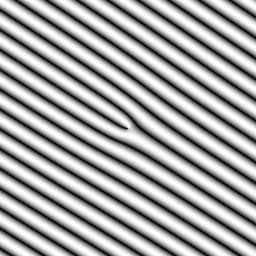
\includegraphics[width=0.235\linewidth]{images/leftSingularity}
  \caption{A simple way to add a single singularity to a sine wave. In order: Phase offset of right singularity, right singularity in Phasor Sine Wave, phase offset of left singularity, left singularity in Phasor Sine Wave. Both Phasor Sine Waves are without wobble. For the phase offsets angle is mapped to hue.}\label{fig:singularities}
\end{figure}

One important thing to note is the fact, that this means, that for each point we need to evaluate each of the singularity terms. For large images with a lot of singularities, this will slow down the evaluation a lot. In such cases, it is common practice to fade out the effects of a local change using a Gaussian function. Once the Gaussian is sufficiently small, the local change can be ignored. However, as Figure \ref{fig:fadedSingularity} shows, this can not be applied here, because our defined function relies on a continuity across the $0$/$2\pi$ boundary. Since the values at this boundary always have to be $0$ and $2\pi$ respectively, we can not simply fade this function out.
\begin{figure}[ht]
  \centering
  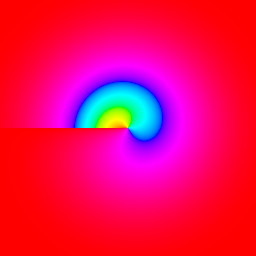
\includegraphics[width=0.49\linewidth]{images/fadedPhase}
  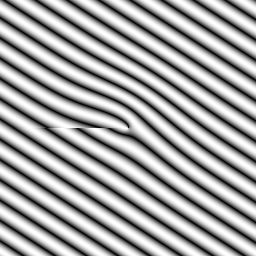
\includegraphics[width=0.49\linewidth]{images/fadedPhaseSineWave}
  \caption{Trying to fade out the phase offset to create a singularity using a Gaussian function. The phase offset (left) is no longer continuous, which leads to a rip in the sine wave (right). Angle is again mapped to hue.}\label{fig:fadedSingularity}
\end{figure}
However, if we take a left and a right singularity and orient them in such a way, that their boundaries point towards each other, we no longer have this problem, as shown in Figure \ref{fig:dualSingularity}. The $0$/$2\pi$ border now has a defined end point. We will call such a pair of singularities a dual singularity. For a pair of Singularities $s_i$ and $t_i$, we can add the following to our generated phase offset:
$$
d(\vec{x}) = ((a(\vec{x})-\pi)\ \mathrm{mod}\ 2\pi)\ b(\vec{x})
$$
with
$$
  a(\vec{x}) = \begin{cases}
  \atan(\vec{x}-\vec{s_i}) - \theta, &\text{if }d_s < d_t\\
  \pi - \atan(\vec{x}-\vec{t_i}) + \theta, &\text{otherwise}
  \end{cases}
$$
and
$$
  b(\vec{x}) = \begin{cases}
    \exp(\frac{d_s^2}{\sigma^2}), &\text{if }d_s < d_t \land d_s < d_l\\
    \exp(\frac{d_t^2}{\sigma^2}), &\text{if }d_t < d_s \land d_t < d_l\\
    \exp(\frac{d_l^2}{\sigma^2}), &\text{otherwise}\\
  \end{cases},
$$
where $\theta=\atan(\vec{t_i}-\vec{s_i})$, $d_s$, $d_t$ and $d_l$ are the distances to $s_i$, $t_i$ and the line connecting the two respectively and $\sigma$ determines the speed at which the dual singularity is faded out. Note that we subtract $\pi$ from this phase offset, to make one side dip down a little, while the other one increase, instead of just one increasing by twice as much. The reason for this is, that to make room for an additional line, the other lines shift slightly as can already be seen in Figure \ref{fig:fadedSingularity} and is still visible in Figure \ref{fig:dualSingularity}. Spreading this shift out to both sides of makes is less visible. Additionally we assume the existence of wobble, which masks this small offset.

\begin{figure}[ht]
  \centering
  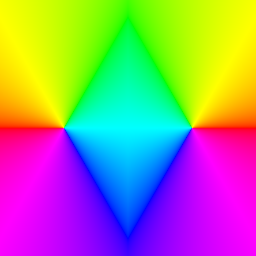
\includegraphics[width=0.32\linewidth]{images/dualSingularityPhase}
  \hfill
  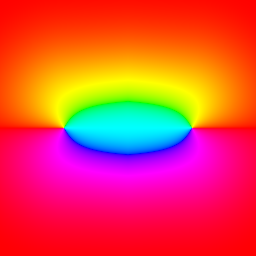
\includegraphics[width=0.32\linewidth]{images/dualSingularityFaded}
  \hfill
  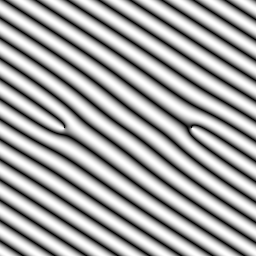
\includegraphics[width=0.32\linewidth]{images/dualSingularitySineWave}
  \caption{The phase offset for a dual singularity (left), the offset for a dual singularity faded by a Gaussian (center) and the phase offset in a sine wave (right).}\label{fig:dualSingularity}
\end{figure}

Using dual singularities, we can expand our constructed phase offset to
\begin{align*}
  \varphi_c(\vec{x})&=w(\vec{x}) +\sum_i d_i(\vec{x})\\
  & + \sum_j \atan(\vec{x}-\vec{s}_j) - \sum_k \atan(\vec{x}-\vec{t_k})
\end{align*}
We use $d_i$ to reference the function to create a dual singularity adapted to $s_i$ and $t_i$. We add the terms for single singularities as there might be a different number of right and left singularities or the use case does not permit the optimization of pairing up all singularities. In an optimal case, one of these sums equals $0$, as there are no summands.

\subsection{Rips}\label{sec:rips}
Rips are caused by a large change in the phase offset. When trying to fade out a single singularity, we already saw, that scaling a $0$/$2\pi$ step creates a large change in phase and by extension a rip. However, when using this technique to create rips, one of the end points can not be controlled easily. In $d(\vec{x})$ we already created a function that creates a $0$/$2\pi$ step along a line connecting two points. Therefore, for a line $l_i$ representing the position for a rip, we can use the corresponding $d_i$ rescaled by a weight $o_i$. Figure \ref{fig:ripPhase} shows the phase of a rip, while Figure \ref{fig:ripWeight} shows the effect the weight has on the rip.

\begin{figure}[ht]
  \centering
  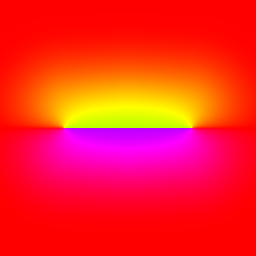
\includegraphics[width=0.49\linewidth]{images/ripPhase}
  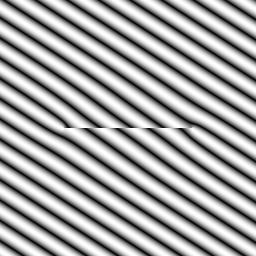
\includegraphics[width=0.49\linewidth]{images/rip05}
  \caption{The phase offset for a rip with a weight of $0.5$ (left) and its impact on a sine wave (right).}\label{fig:ripPhase}
\end{figure}

\begin{figure}[ht]
  \centering
  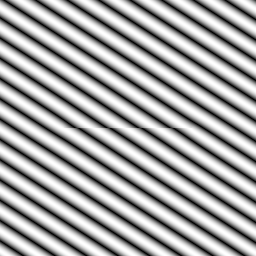
\includegraphics[width=0.32\linewidth]{images/rip01}
  \hfill
  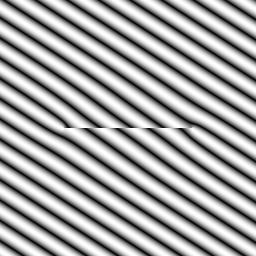
\includegraphics[width=0.32\linewidth]{images/rip05}
  \hfill
  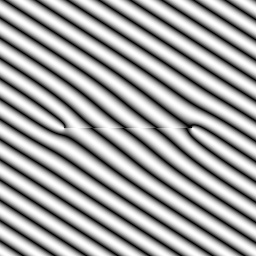
\includegraphics[width=0.32\linewidth]{images/rip09}
  \caption{A rip with a weight of $0.1$ (left), one with a weight of $0.5$ (center) and one with a weight of $0.9$ (right). The low weight of the first rip leads to an almost negligible rip, while the medium weight of the second leads to the maximum difference between the sides of the rip. The large weight of the last also leads to only a small offset. However, the rip is framed by singularities on both sides.}\label{fig:ripWeight}
\end{figure}

\begin{figure}[ht]
  \centering
  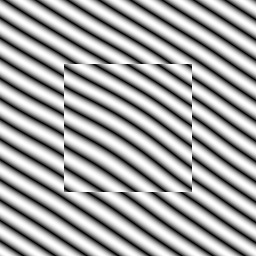
\includegraphics[width=0.49\linewidth]{images/ripChaining}
  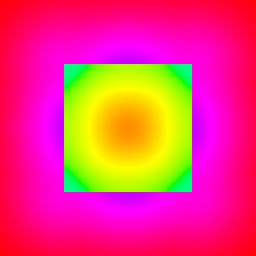
\includegraphics[width=0.49\linewidth]{images/ripChainingPhase}
  \caption{Multiple rips chained together to form a square (left) and the phase offset used to accomplish this (right).}\label{fig:ripChaining}
\end{figure}

As Figure shows, \ref{fig:ripChaining} rips can be chained without additional artifacts to generate more complex shapes.\\
Using this, we can once again expand our constructed phase offset:
\begin{align*}
  \varphi_c(\vec{x})&=w(\vec{x}) +\sum_i d_i(\vec{x})\\
  & + \sum_j \atan(\vec{x}-\vec{s}_j) - \sum_k \atan(\vec{x}-\vec{t_k})\\
  & + \sum_l w_l\cdot d_l(\vec{x}),
\end{align*}
where $d_l$ is the dual singularity function corresponding to the endpoints of $l_l$ and $w_l$ is the weight for $l_l$.\\
\\
For demonstration purposes, we always used only one artifact type at a time, however the different artifact type can be freely combined as Figure \ref{fig:combiningArtifacts} shows.

\begin{figure}[ht]
  \centering
  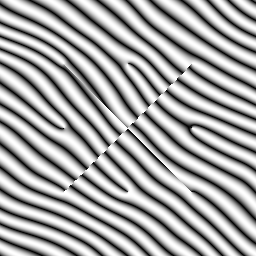
\includegraphics[width=0.49\linewidth]{images/combiningArtifacts}
  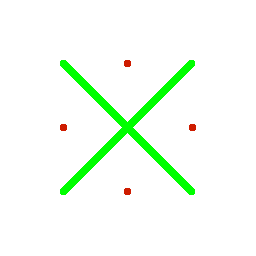
\includegraphics[width=0.49\linewidth]{images/combiningArtifactsPositions}
  \caption{A combination of multiple artifacts (left) and the position of the artifacts fed to the algorithm (right). The positions for singularities are marked in red, while the positions for rips are marked in green. This combination does not create any unwanted artifacts.}\label{fig:combiningArtifacts}
\end{figure}



\section{The non-constant Case}\label{sec:nonConstant}
The second case we will look at is the more general non-constant one. In this context non-constant refers to the stripe direction and frequency. The main difficulty with this is to find a base function, that increases orthogonally to the stripe direction, that can be used as a basis for the phase. In general, this function is the integral of the direction field. In the constant case, this direction field was constant, so the integral was a linear function. However, not all vector fields are integrable and therefore we need to differentiate between the two cases.

\subsection{Integrable Direction Field}
We will first look at the case, where the direction field is integrable. Knowing a function whose derivative is the direction field we want to use makes it possible to use all the concepts we went over in the previous sections. For the integral $I(\vec{x})$ of the direction field, we can replace the linear function $f\langle\vec{x},\vec{u}\rangle$ with $I(x)$ to receive:
$$
P_c(\vec{x}) = \sin(I(\vec{x})+\varphi_c(\vec{x}))
$$
Figure \ref{fig:parabola} shows a Phasor noise instance using the direction field
$$
d(\vec{x}) = \begin{pmatrix}
2x_1+x_2^2\\
x_1^2+2x_2
\end{pmatrix},
$$
which integrates to
$$
I(\vec{x}) = x_1^2 + x_2^2 = \langle \vec{x},\vec{x} \rangle.
$$

\begin{figure}[ht]
  \centering
  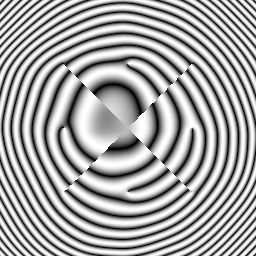
\includegraphics[width=0.49\linewidth]{images/paraboloidDir}
  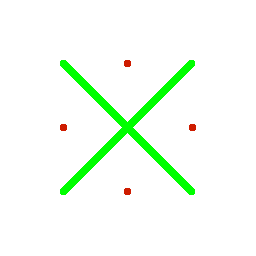
\includegraphics[width=0.49\linewidth]{images/combiningArtifactsPositions}
  \caption{A constructed Phasor noise instance using the derivative of a parabola as direction field (left) and the positions of the artifacts (right). The positions for singularities are shown in red and the positions of for rips are shown in green.}\label{fig:parabola}
\end{figure}

\subsection{Non-integrable Direction Field}\label{sec:stripes}
A case with a non-integrable direction field is much harder, as we can not simply integrate the direction field to obtain the base for the sine wave. However, \cite{stripes} develops a substitute for this base function, we will call $f(\vec{x})$. The technique already presents a way to prescribe singularities, so we will not have a look at singularities in this section. Even if we do not add any singularities, some direction fields require some, so it may not be possible to avoid them. Another major limitation of this technique is the requirement to use an oscillation profile, that is symmetric to the $y$-axis. We can try to use a cosine based oscillation instead of a sine based one. However, since adding a phase to a cosine is equal to shifting it along the $x$-axis, we can not add a phase offset without creating artifacts in the image.\\
One method to create a base function, which we can use, is to create a low frequency oscillation and create a symmetric, but locally different function. Another way to express this approach is to use one period of the created function to create multiple stripes in the output. However, as Figure \ref{fig:multiStripe} shows, this massively amplifies the effect of the already existing singularities. Apart from this, this approach can be used as the others, so we will not discuss it further.

\begin{figure}[ht]
  \centering
  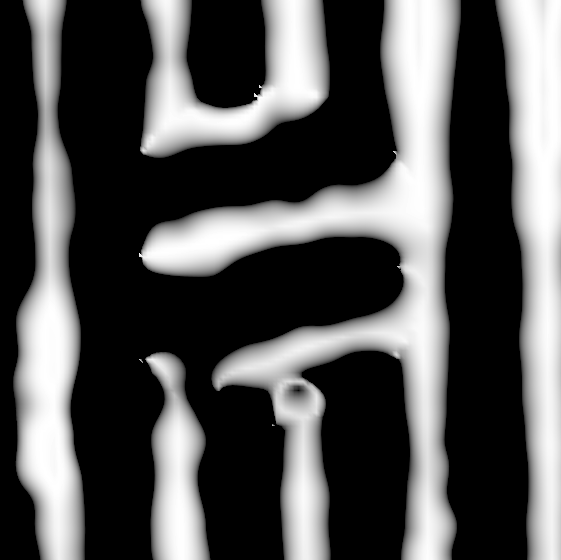
\includegraphics[width=0.49\linewidth]{images/multiStripe}
  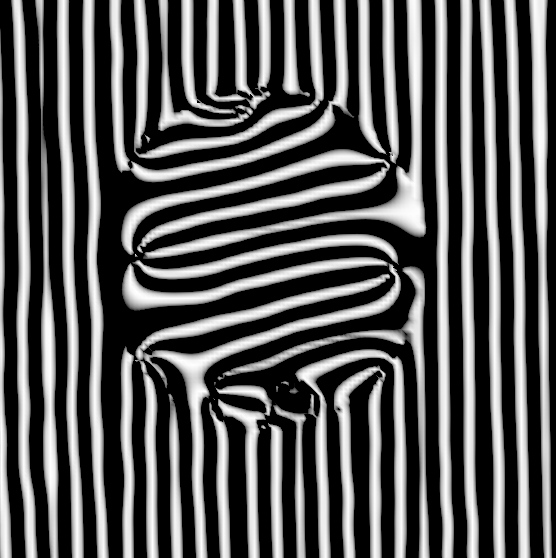
\includegraphics[width=0.49\linewidth]{images/multiStripeMulti}
  \caption{A low frequency stripe pattern with varying direction and wobble (left) and the pattern extended to create multiple stripes per period (right).}\label{fig:multiStripe}
\end{figure}

Another approach is to try to adapt the techniques we developed so far to work with these limitations. However, as we will see, this too will not be as successful as in the constant case. As before, the first artifact we will have a look at is wobble. We apply a simple trick to ensure the symmetry of our function. The first thing we do is to take the absolute value of $f$. We will now add wobble as we did before. The result is shown in Figure \ref{fig:multiDirWobble}. Instead of the lines moving to one side, they actually vary in width. This is because we do not know on which side of the peak we are, so we can either add or subtract from both. Of course, the actual value varies, but since the wobble phase offset is continuous, so in a local area, it is either one or the other.

\begin{figure}[ht]
  \centering
  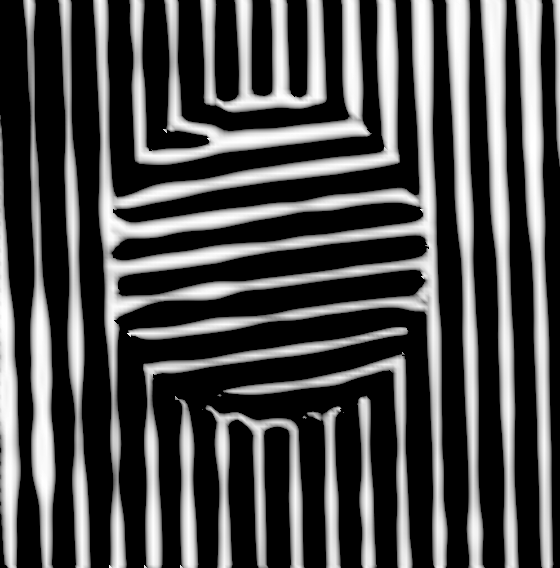
\includegraphics[width=0.49\linewidth]{images/multiDirWobble}
  \caption{Adding wobble does not move the lines, but causes them to vary in width.}\label{fig:multiDirWobble}
\end{figure}

The other artifact type we will have a look at is rips. Having a look at Figure \ref{fig:multiDirRip}, it is apparent, that again the forced symmetry is problematic, as the lines do not shift to create an offset, but vary in width. It still creates something akin to a rip.

\begin{figure}[ht]
  \centering
  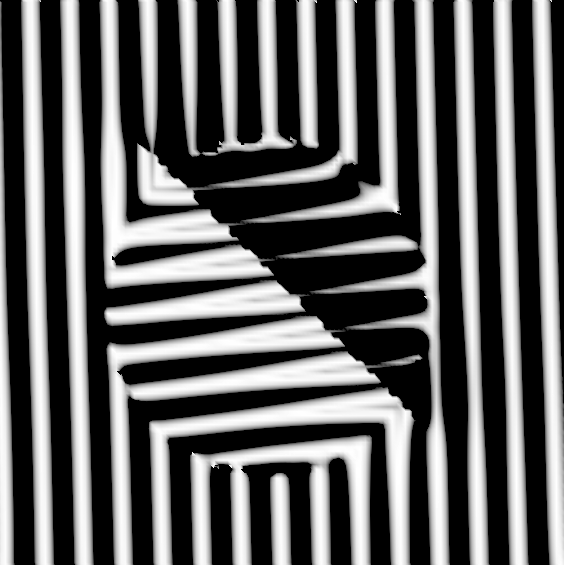
\includegraphics[width=0.49\linewidth]{images/multiDirRip}
  \caption{Creating a rip in an environment with a non-integrable direction field. The lines do not shift to create an opposition, but vary in width.}\label{fig:multiDirRip}
\end{figure}

\section{Results}\label{sec:results}
Our technique naturally lends itself to applications Phasor noise is useful in, especially if only some artifact types are wanted. Figure \ref{fig:mountains} shows a mountain range generated using wobble and randomly placed singularities. It also shows how a prescribed rip can be used to mimic offset in the terrain created by an earthquake. Figure \ref{fig:desert} also makes use of a prescribed rip to emulate sand dunes, that form around a sheet of glass. Another interesting application of rips is shown in Figure \ref{fig:bricks}, where a constructed Phasor noise instance is used to create detail in a texture, that respects the existing boundaries of the texture.

\begin{figure}[ht]
  \centering
  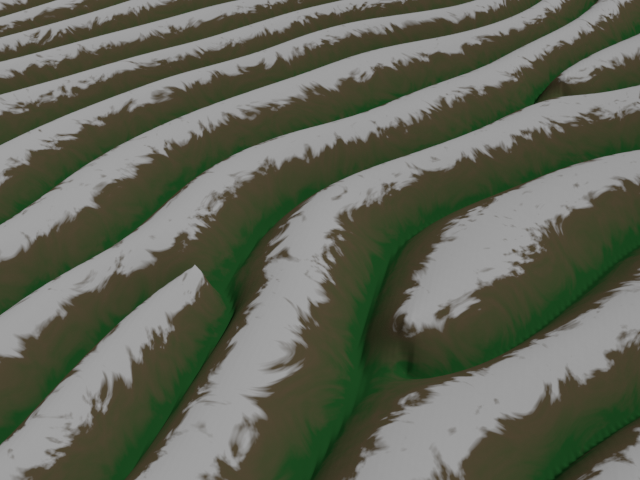
\includegraphics[width=\linewidth]{images/mountains}

  \vspace{2pt}
  
  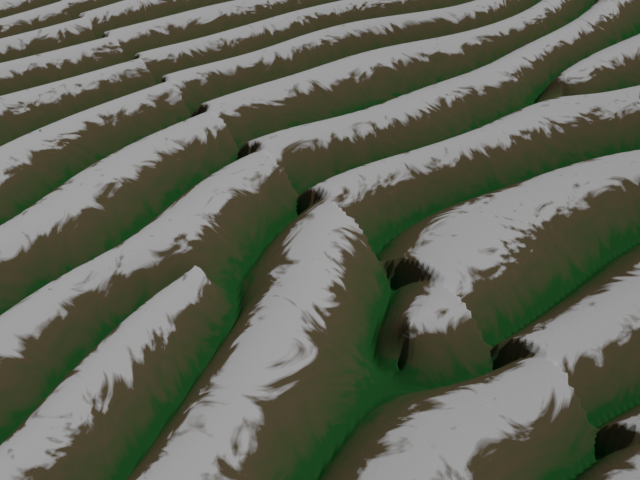
\includegraphics[width=\linewidth]{images/mountainsRip}
  \caption{A procedurally generated mountain range using wobble and singularities (top) and the same mountain range disturbed by an earthquake (bottom).}\label{fig:mountains}
\end{figure}

\begin{figure}[ht]
  \centering
  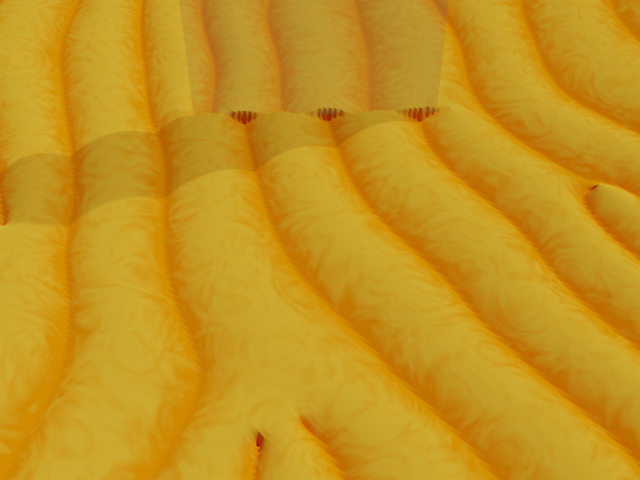
\includegraphics[width=\linewidth]{images/desert}
  \caption{Procedurally generated dunes in a desert forming around a sheet of glass. Where the glass intersects the sand, a rip was placed to cause a discontinuity in the pattern.}\label{fig:desert}
\end{figure}

\begin{figure}[ht]
  \centering
  
\includegraphics[width=0.49\linewidth]{images/brick}
  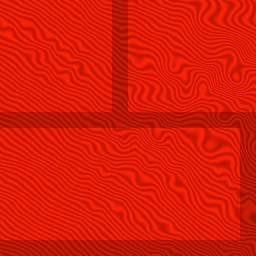
\includegraphics[width=0.49\linewidth]{images/brickSimple}

  \vspace{2pt}

  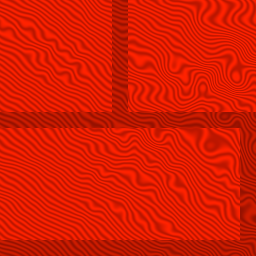
\includegraphics[width=0.49\linewidth]{images/brickRespecting}
  \caption{Adding detail to a na\"ively upscaled marble brick texture. The original texture (left) and a version with na\"ively added detail (center). We can use rips to force discontinuities where the original texture suggests a change of material (right). In this case this is at the edges between the white and grey parts of the texture.}\label{fig:bricks}
\end{figure}

\section{Future Work}
Despite the demonstrated use cases for constructed artifacts in Phasor noise and the lack thereof, there are still more areas to explore. One of these areas is the non-constant case. While the integrable case works fine, the non-integrable case still needs more work. The main limitation is the fact, that asymmetric oscillation profiles are not possible. On one hand, we could try to keep track of where in the period we are, to enable asymmetric oscillation profiles, while on the other hand we could try to adapt the methods described here to work with symmetric oscillation profiles. Finding a good way to work with the work presented in \cite{stripes} also enables the application of this approach to work as surface noise. While this leads to a need for texture coordinates to specify where on the object artifacts should appear, these do not have to be free of discontinuities, as they would only be used for this purpose. Therefore, even simple algorithms that generate texture coordinates will do.\\
Another avenue, that can be explored, is an adaptation to work in higher dimensions, especially in a three dimensional environment. For the integrable case, this is can be done by defining three dimensional equivalents to the artifact generation functions we defined here. The non-integrable case also requires the definition of a function, that can be used as a base for the oscillation.

\section{Conclusion}
In the integrable case, we can now freely control the artifacts Phasor noise exhibits. We can do this by constructing the phase using a linear function as a base. We then proceed to add constructed functions, that correspond to the artifact types and positions we want. Using a periodic function, we can than convert this to a Phasor noise instance. We also has a look at how the non-integrable case can be handled, where the difficulty lies in finding a base that is consistent with the given direction field. The presented method allows the automated creation of new types of content, as we have seen. These additional automation opportunities will aid in the never ending fight against shorter development cycles.


\FloatBarrier
\printbibliography


\end{document}

